\documentclass[compress,aspectratio=169]{beamer}


%%%--- beamer ---%%%
\usetheme{Nice}
%\usetheme{Singapore}
\usecolortheme{rose}

%%%--- Details on Document ---%%%
\author{B. Carry \& M. Mahlke}
\institute{Les Houches PNP school}
\date{2024}
\title{Online Tools in Planetary Sciences - Part II}

%%%--- Hyperreferences ---%%%%
\usepackage{hyperref}
\hypersetup{
%%%%--- Options for Acrobat
    bookmarks=true,         % show bookmarks bar?
    unicode=true,           % non-Latin characters in Acrobat's bookmarks
    pdftoolbar=true,        % show Acrobat's toolbar?
    pdfmenubar=true,        % show Acrobat's menu?
    pdffitwindow=true,      % page fit to window when opened
%%%%--- PDF informations
    pdfauthor={B. Carry},
    pdfkeywords={},         % list of keywords
%%%%--- Link option
    pdfnewwindow=true,      % links in new window
    colorlinks=true,        % false: boxed links; true: colored links
    linkcolor=gray,         % color of internal links
    citecolor=blue,         % color of links to bibliography
    filecolor=gray,         % color of file links
    urlcolor=gray           % color of external links
}


%%%--- Graphics and Colors ---%%%
\usepackage{tabularx}
\usepackage{graphicx}
\usepackage{color}
\graphicspath{{gfx/}}
\definecolor{ERCblue}{HTML}{004d95}
\definecolor{ERCpurple}{HTML}{800080}

%%%--- Useful commands---%%%
\newcommand{\etal}{\textsl{et al.}}
\newcommand{\degr}{\ensuremath{^\circ}}
\newcommand{\arcsec}{\mbox{\ensuremath{^{\prime\prime}}}}

\renewcommand{\emph}[1]{\textcolor{ERCblue}{#1}}
\newcommand{\strong}[1]{\textcolor{ERCpurple}{#1}}
\newcommand{\src}[1]{\textcolor{gray}{\tiny #1}}
\newcommand{\param}[1]{\textcolor{gray}{\texttt{#1}}}

%%%--- For editing amongst teachers ---%%%
\newcommand{\MM}[1]{\textbf{\textcolor{cyan}{#1}}}
\newcommand{\BC}[1]{\textbf{\textcolor{purple}{#1}}}
\newcommand{\tbd}[1]{\textbf{\textcolor{red}{#1}}}


%%%--- beamer setup ---%%%
\setbeamertemplate{navigation symbols}[only frame symbol]
\setbeamertemplate{blocks}[rounded][shadow=false]

%%%--- main ---%%%
\begin{document}

  %%%%%%%---- BEGIN ---- Title frame ----%%%%%%
\begin{frame}

  \begin{center}

    \emph{\Large Online tools for planetary sciences}\\

    \vspace{2em}
    \begin{columns}[T]
      \begin{column}{.3\textwidth}
        \vspace{0.5em}
\includegraphics[width=.5\textwidth]{logo-ivoa}\\
        \vspace{0.5em}
\includegraphics[width=.5\textwidth]{logo-sbpy}\\
        \vspace{0.5em}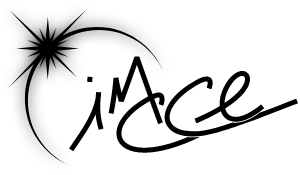
\includegraphics[width=.5\textwidth]{logo-imcce}\\
        \vspace{0.5em}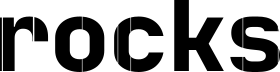
\includegraphics[width=.5\textwidth]{logo-rocks}
      \end{column}
      %      
      \begin{column}{.7\textwidth}
        \small
        \vspace{3cm}
        \textbf{B.~Carry}$^1$ \&
        \textbf{M.~Mahlke}$^2$\\
        \footnotesize{$^1$Lagrange, Observatoire de la C{\^o}te d'Azur, Nice}\\
        \footnotesize{$^1$Institut d'Astrophysique Spatiale, Orsay}
      \end{column}
    \end{columns}

  \end{center}

\end{frame}
%%%%%%%----  END  ---- Title frame ----%%%%%%
         %-Ok
  \section{Data Access}
\label{sec:databases}

%%%%%%%---- BEGIN ----  ----%%%%%%
\begin{frame}
  \frametitle{Databases and Data Aggregators}

  \begin{columns}[T]

      \begin{column}{.3\textwidth}
        \only<1>{%
          \vspace{0.5em}
\includegraphics[width=.8\textwidth]{logo_cds}\\
          \vspace{0.5em}
\includegraphics[width=.8\textwidth]{logo_pds}\\
          % \vspace{0.5em}
\includegraphics[width=.8\textwidth]{logo_mp3c}\\
          % \vspace{0.5em}
\includegraphics[width=.8\textwidth]{logo_ssodnet}\\
        }%
        \only<2->{%
          \vspace{0.5em}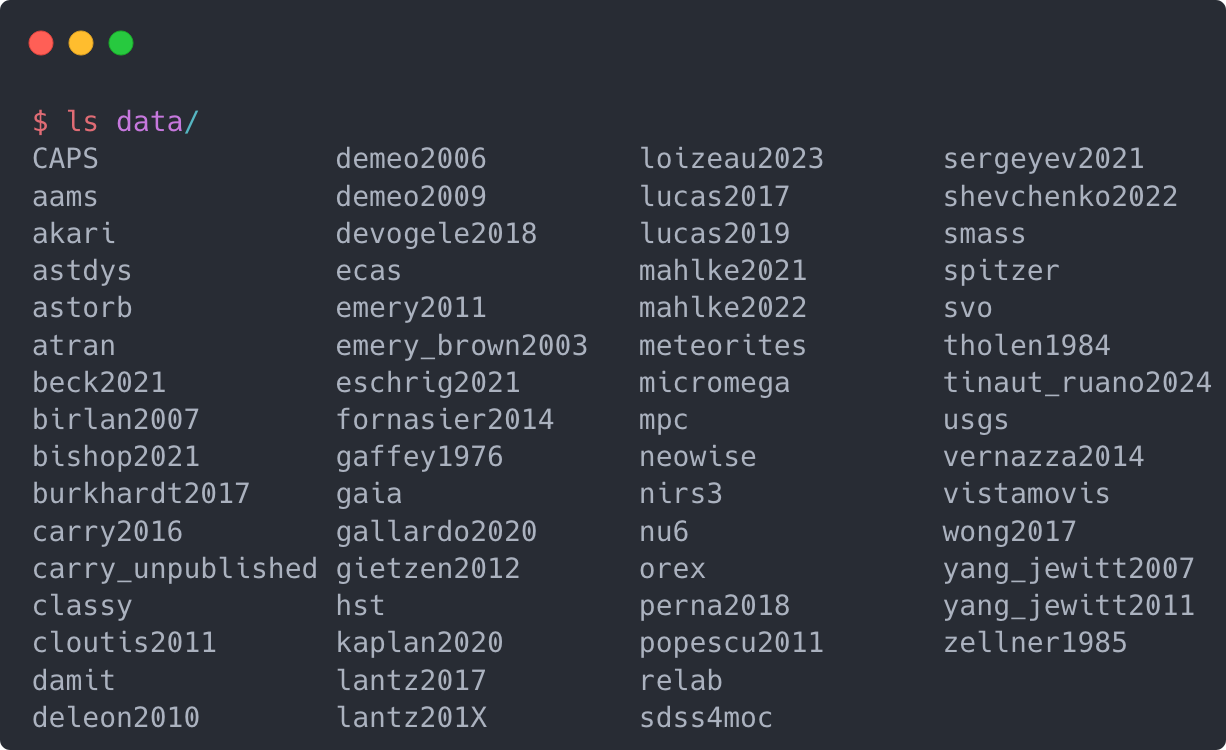
\includegraphics[width=.8\textwidth]{data_dir}\\
          \vspace{0.5em}
\includegraphics[width=.8\textwidth]{logo_astorb}\\
          \vspace{0.5em}
\includegraphics[width=.8\textwidth]{logo_mp3c}\\
          \vspace{0.5em}
\includegraphics[width=.8\textwidth]{logo_ssodnet}\\
        }%
      \end{column}


    \begin{column}{.7\textwidth}
      \begin{overlayarea}{\textwidth}{\textheight}
          \vspace{1em}
          We all need data, we all generate data.\\
          \vspace{1em}
          \begin{itemize}[<.->]
            \item \emph{\bf Databases}
              \begin{itemize}[<.->]
                \item[$\circ$] Websites, CDS, on request
                \item[$\circ$] Mostly static, single bibliographic reference
                \item[$\circ$] Mixture of formats
              \end{itemize}

            \only<2->{%
            \vspace{0.5em}
            \item \emph{\bf Data Aggregators}
              \begin{itemize}[<.->]
                \item[$\circ$] Collection of data \emph{with processing}
                \item[$\circ$] Dynamic, large number of bibliography references
                \item[$\circ$] Uniform output
              \end{itemize}
            }%
          \end{itemize}

          \only<3->{%
          \vspace{0.5em}
          Data aggregation takes effort but saves time and energy.
          }%
      \end{overlayarea}
    \end{column}

  \end{columns}

\end{frame}

\begin{frame}[t]
  \frametitle{Data Aggregators}
  {\scriptsize
  \begin{table}[t]
    \begin{tabular}{llll}
      \textsc{Name} & \textsc{Objects} & \textsc{Parameters} & \textsc{URL} \bigskip\\
      ECOCEL & Asteroids & Physical, Orbital &  \tiny \url{http://www.ecocel-database.com/}\smallskip\\
      JPL SBDB & Asteroids, Comets & Physical, Orbital & \tiny \url{https://ssd.jpl.nasa.gov/tools/sbdb_lookup.html}\smallskip\\
      Lowell & Asteroids & Physical, Orbital &  \tiny\url{https://asteroid.lowell.edu/astinfo/}\smallskip\\
      MP3C & Asteroids & Physical, Orbital &  \tiny\url{https://mp3c.oca.eu/}\smallskip\\
      NEOExchange & Near-Earth Objects & Orbital &  \tiny\url{https://neoexchange.lco.global/}\smallskip\\
      SiMDA & Asteroids, Comets & Size, Mass, Density & \tiny \url{https://astro.kretlow.de/simda/}\smallskip\\
      SsODNet & Asteroids & Physical, Orbital & \tiny \url{https://ssp.imcce.fr/forms/ssocard}\smallskip\\
    \end{tabular}
  \end{table}
  }
\end{frame}

\begin{frame}[t]{Demo}
  The next slides show an outline of the demoed material.
\end{frame}

\begin{frame}[t]{Demo}
  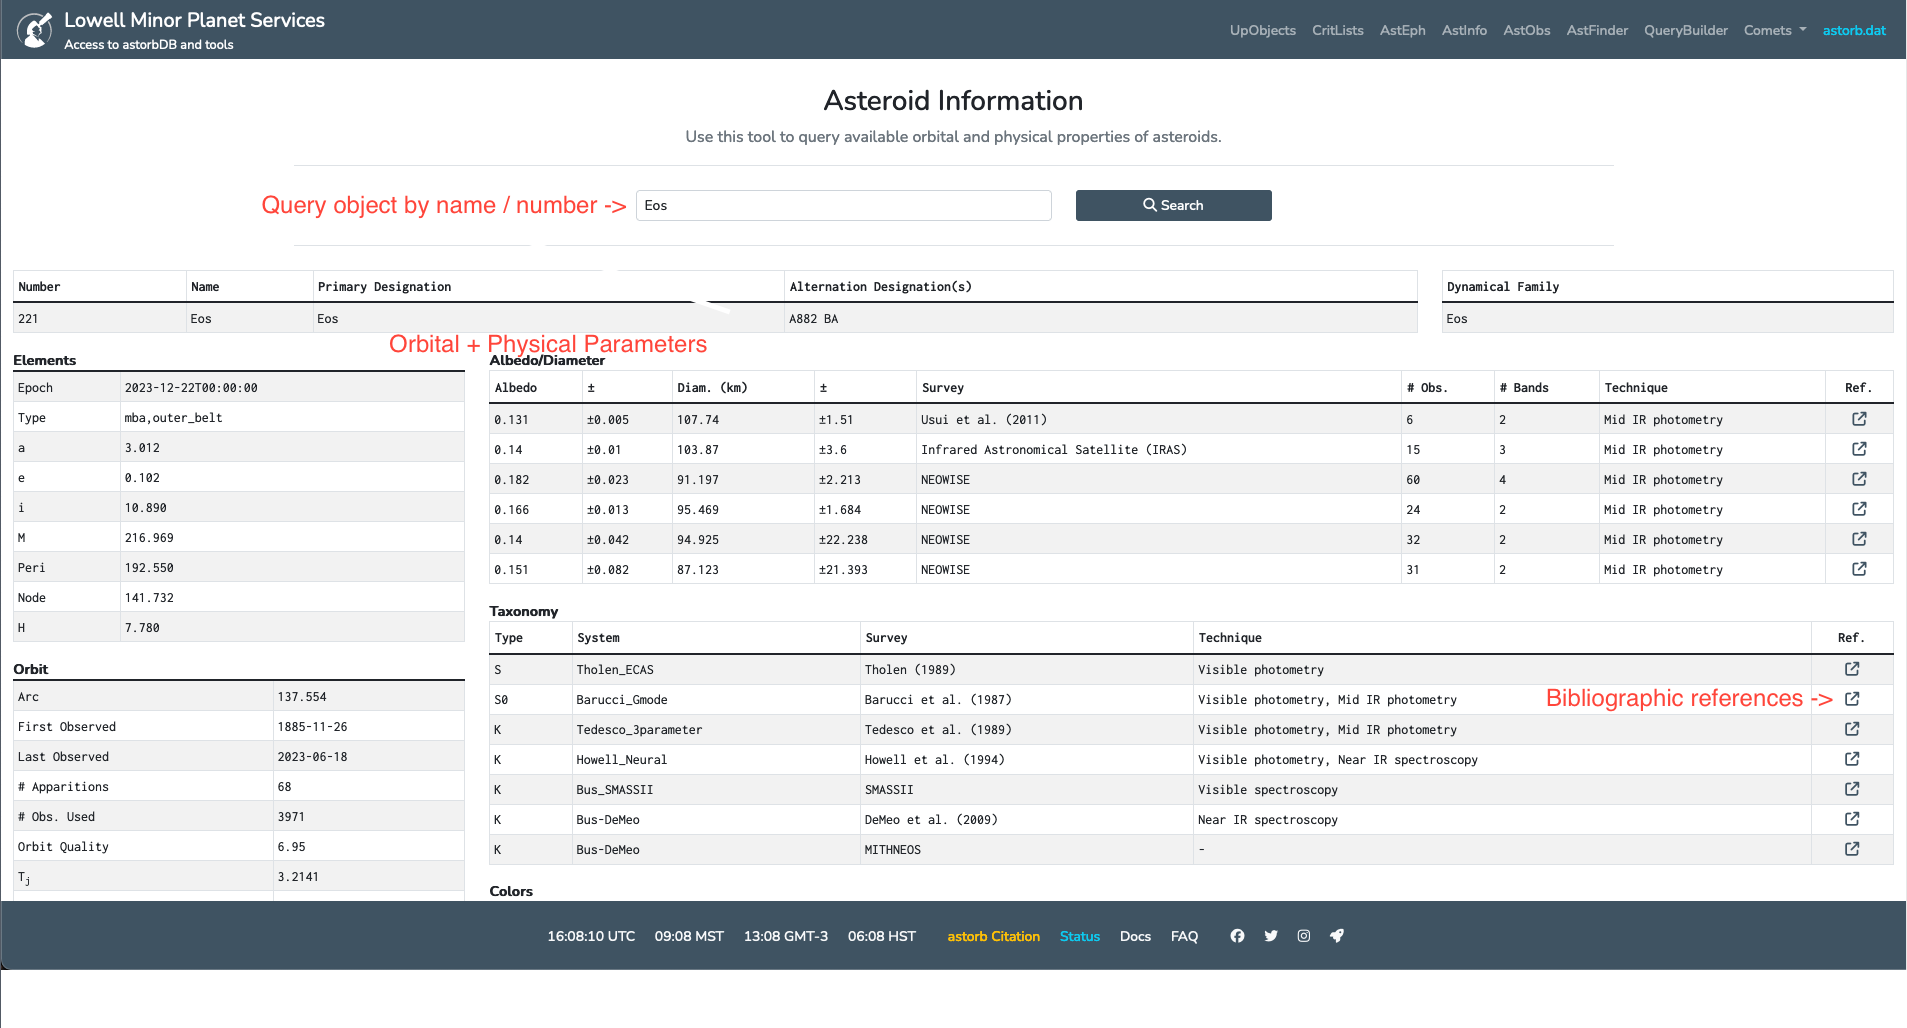
\includegraphics[width=0.9\textwidth]{gfx/demo_lowell.png}
  \url{https://asteroid.lowell.edu/}
\end{frame}

\begin{frame}[t]{Demo}
  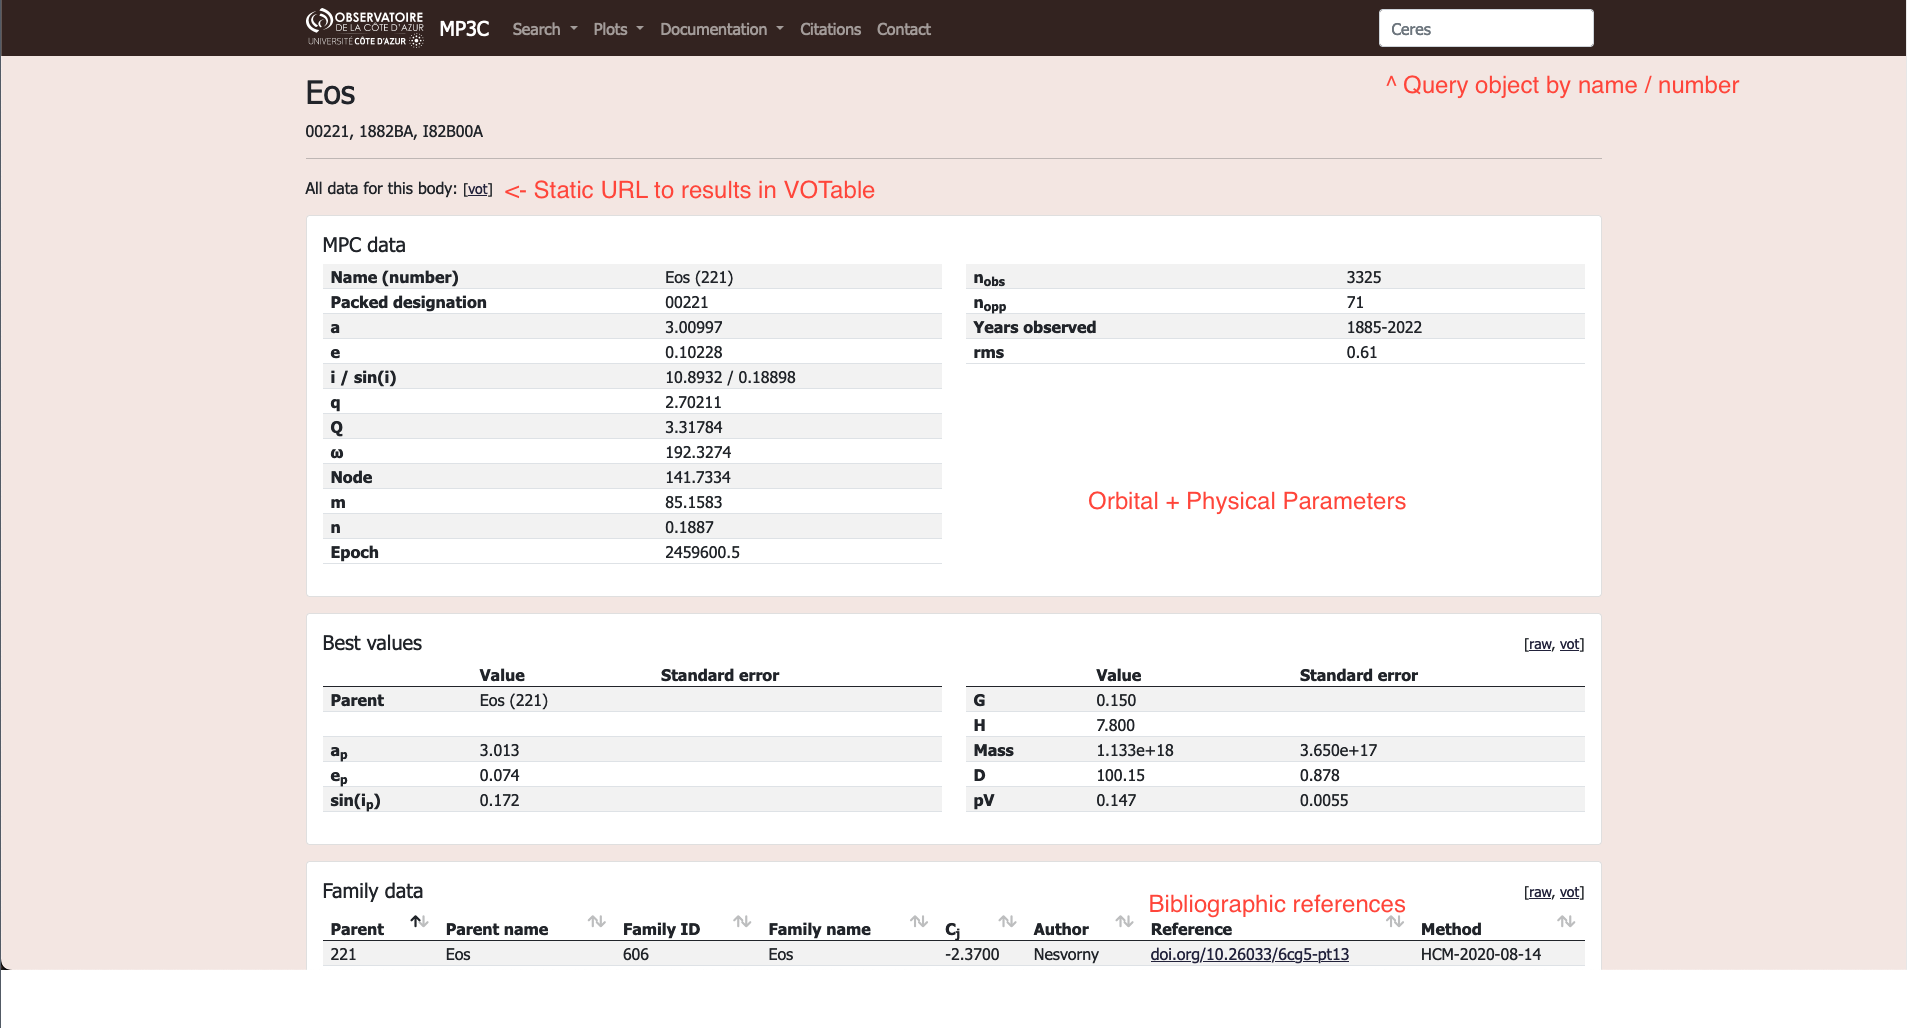
\includegraphics[width=0.9\textwidth]{gfx/demo_mp3c.png}
  \url{https://mp3c.oca.eu/}
\end{frame}

\begin{frame}[t]{Demo}
  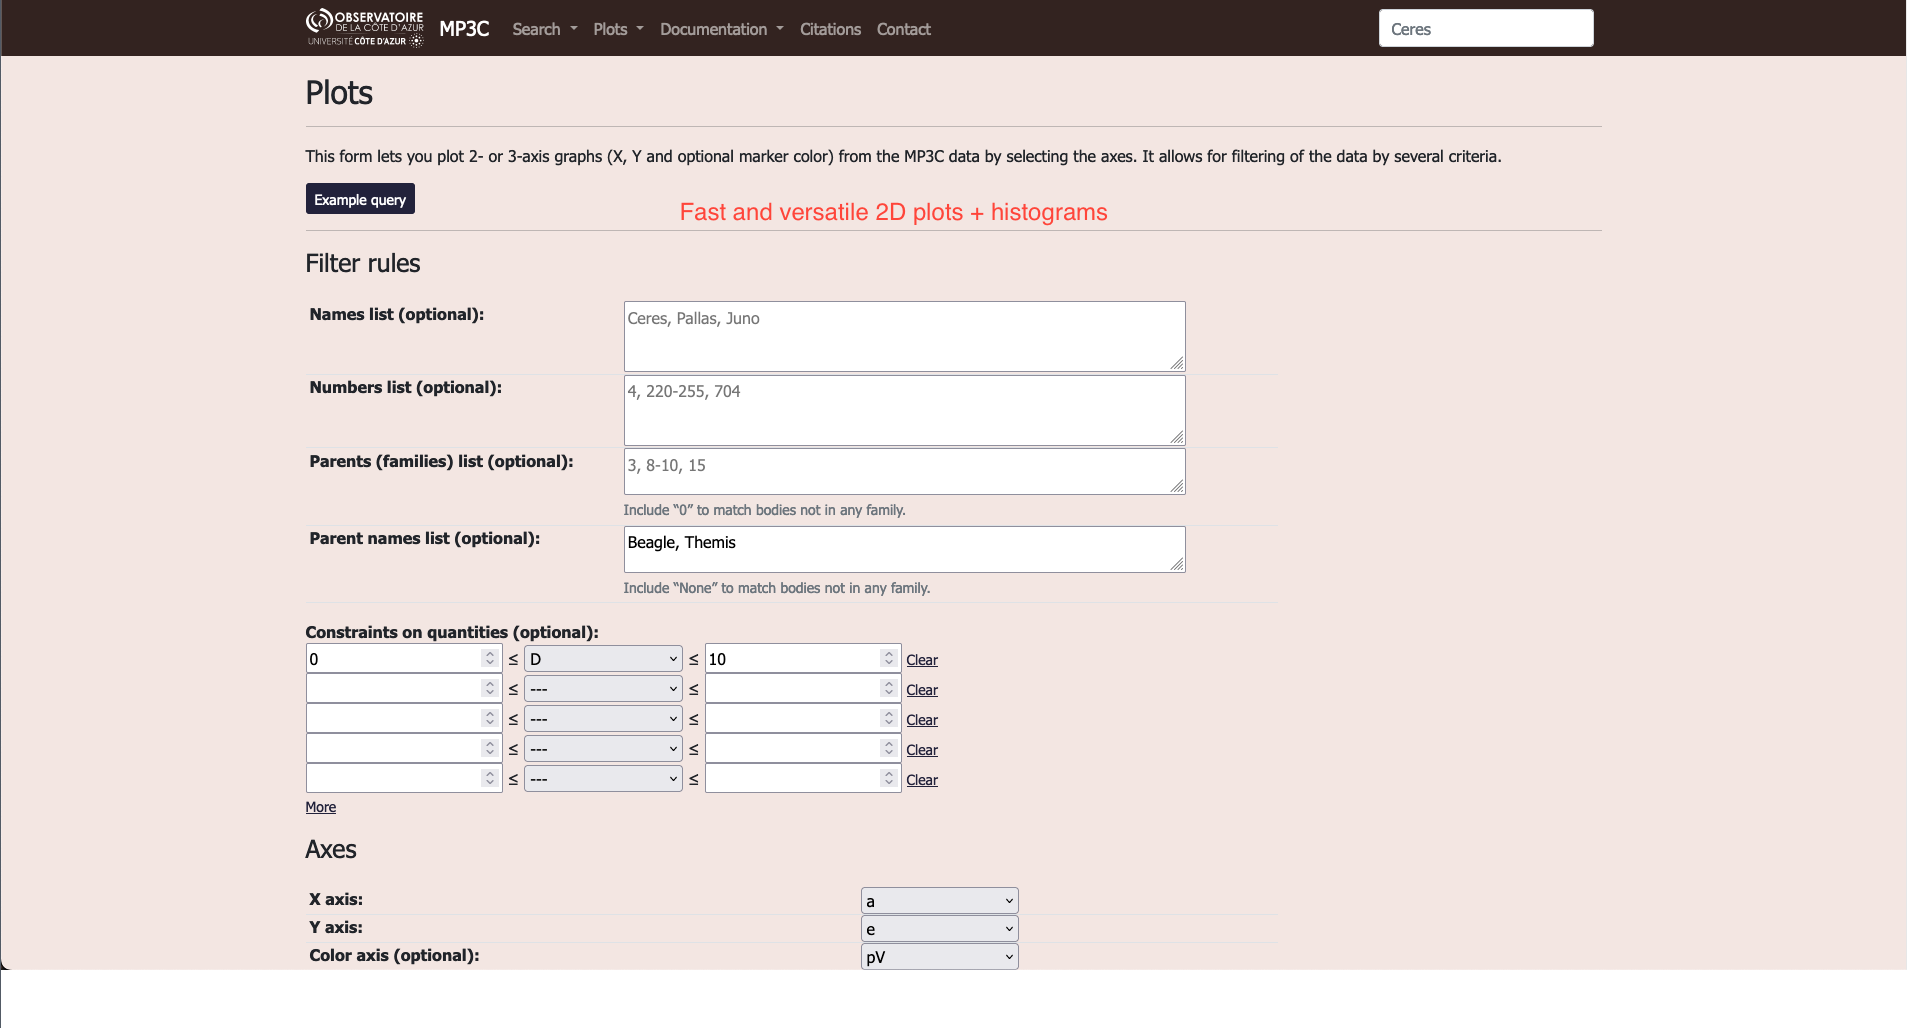
\includegraphics[width=0.9\textwidth]{gfx/demo_mp3c_2.png}
  \url{https://mp3c.oca.eu/xyc-plot/}
\end{frame}

\begin{frame}[t]{Demo}
  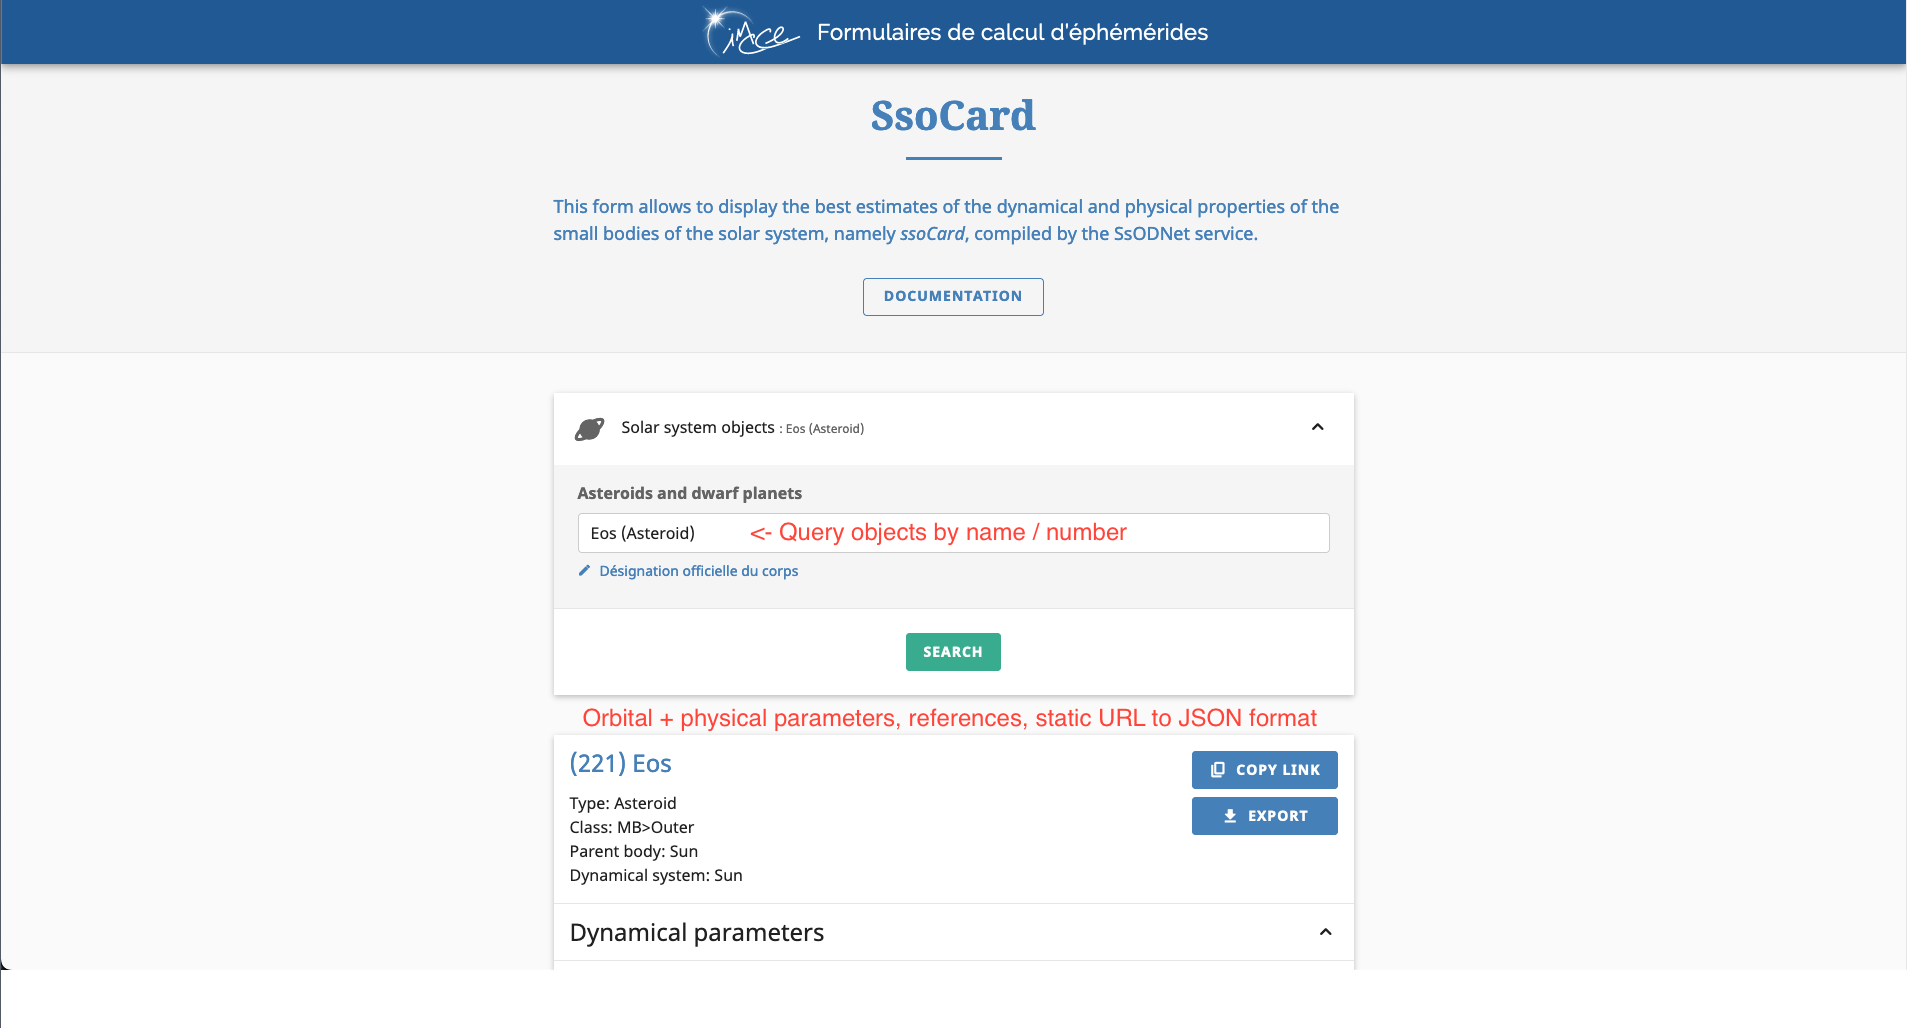
\includegraphics[width=0.9\textwidth]{gfx/demo_ssocard.png}
  \url{https://ssp.imcce.fr/forms/ssocard}
\end{frame}

\begin{frame}[t]{Demo}
  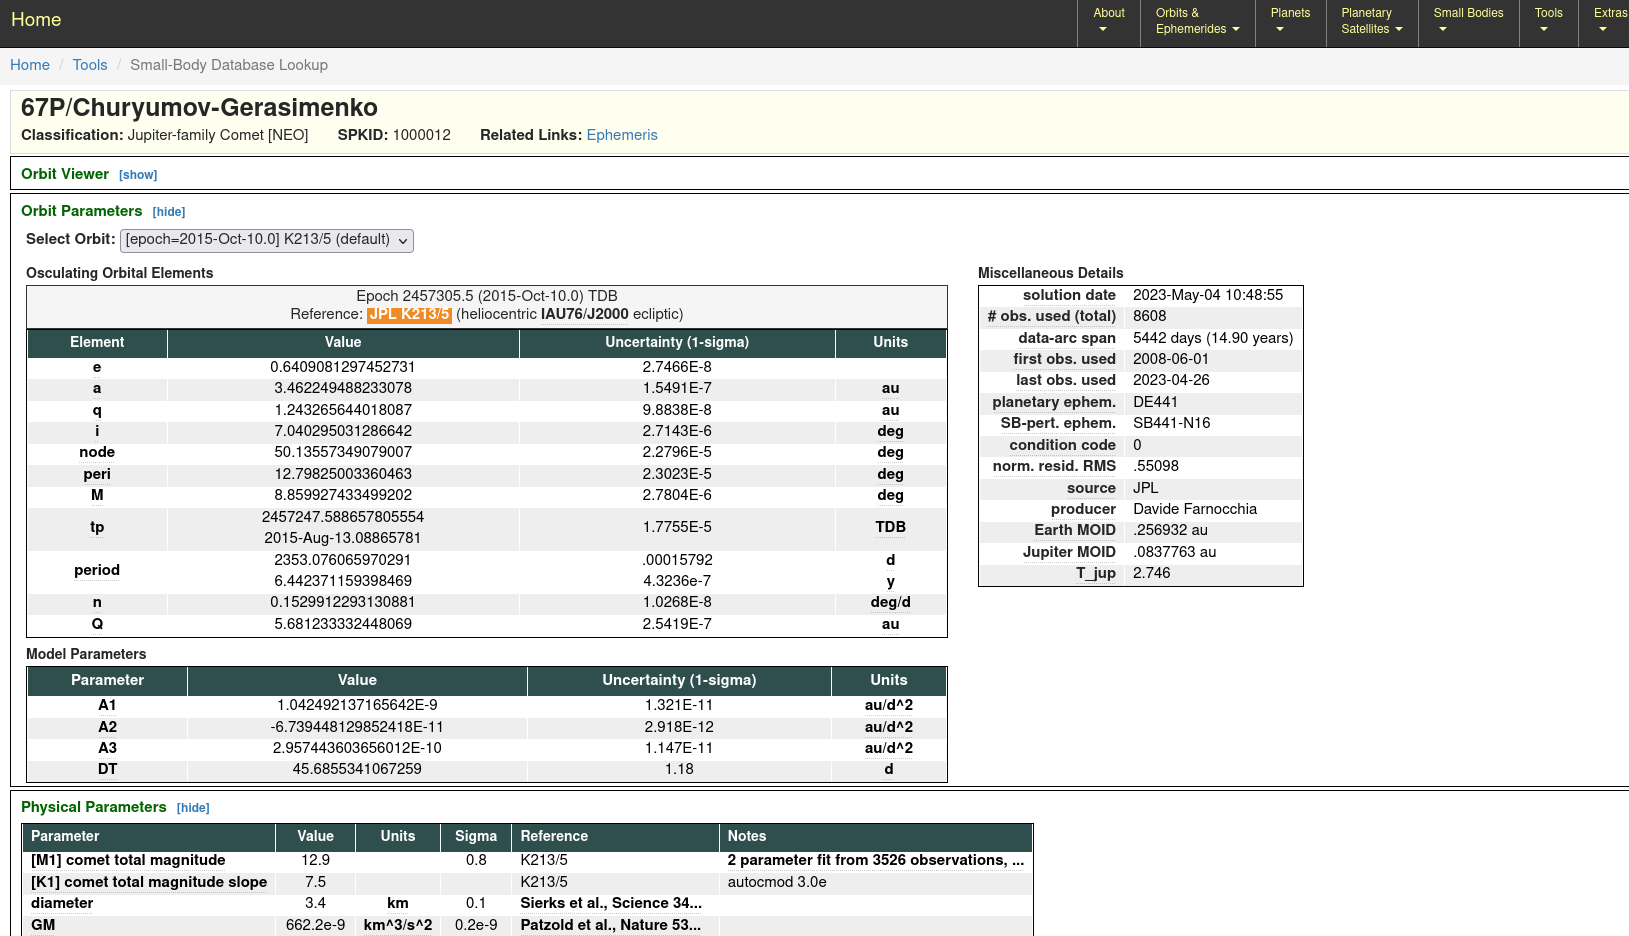
\includegraphics[width=0.8\textwidth]{gfx/demo_jpl.png}
  \url{https://ssd.jpl.nasa.gov/tools/sbdb_lookup.html}
\end{frame}

\begin{frame}[t]{Data Aggregators}
    And the meteorites?
    \smallskip
    \begin{itemize}
      \item Meteoritical Bulletin {\tiny\url{https://www.lpi.usra.edu/meteor/}}
        \begin{itemize}
          \item Name, classification, fall/find
          \item Meteorite Name Checking Utility {\tiny\url{https://www.lpi.usra.edu/meteor/metbullcheck.php}}
        \end{itemize}
        \vspace{0.5em}
      \item Antarctic Meteorite Classification Database {\tiny\url{https://curator.jsc.nasa.gov/antmet/}}
        \begin{itemize}
          \item[$\circ$] Has an API :-)
          \item[$\circ$] Only records antarctic meteorites :-(
        \end{itemize}
    \end{itemize}

    \only<2->{
      \bigskip
      Need for a meteorite database + API!
    }
\end{frame}

\begin{frame}[t]{The N-Body Problem}

\begin{columns}[T]

      \begin{column}{.3\textwidth}
        \vspace{0.5em}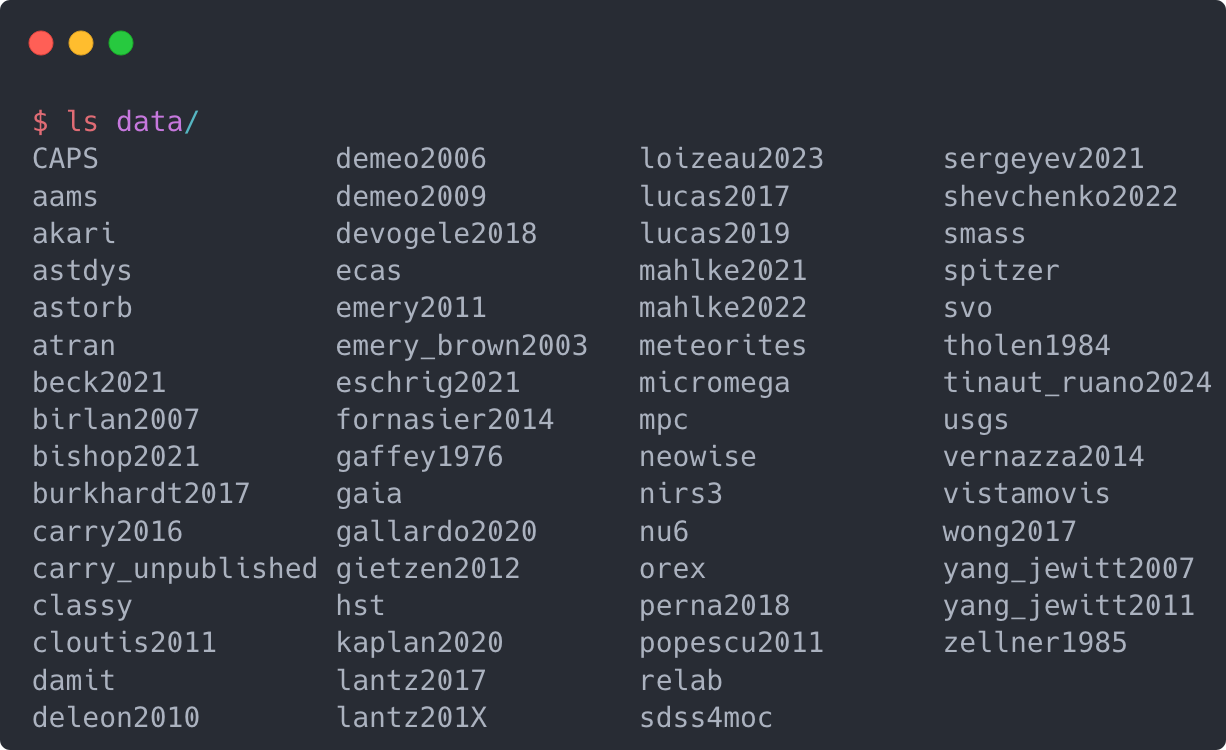
\includegraphics[width=.8\textwidth]{data_dir}\\
        \vspace{0.5em}
\includegraphics[width=.8\textwidth]{logo_astorb}\\
        \vspace{0.5em}
\includegraphics[width=.8\textwidth]{logo_mp3c}\\
        \vspace{0.5em}
\includegraphics[width=.8\textwidth]{logo_ssodnet}\\
      \end{column}

    \begin{column}{.7\textwidth}
      \begin{overlayarea}{\textwidth}{\textheight}

        %
        % We access the same data for many objects multiple times.
        \begin{itemize}[<.->]
          \item \emph{\bf Graphical User Interfaces do not scale}
            \begin{itemize}[<.->]
              \item[$\circ$] Many bodies \textrightarrow~Many clicks
              \item[$\circ$] Repeated queries to update data
              \item[$\circ$] Bibliography management
            \end{itemize}
        \end{itemize}
          \textrightarrow~Data aggregators need programmatic APIs

      \vspace{1.0em}
        \begin{itemize}[<.->]
          \item \emph{\bf Different degrees of simplification}
            \begin{itemize}[<.->]
              \item[$\circ$] Static URLs pointing to text files
              \item[$\circ$] Common service such as the \textit{Table Access Protocol}
              \item[$\circ$] Secondary client such as \texttt{python} packages
            \end{itemize}
        \end{itemize}
      \vspace{0.5em}
        % \begin{itemize}[<.->]
        %   \item[\textrightarrow] \emph{\bf We need to know how to use them}
        %     \begin{itemize}[<.->]
        %       \item[$\circ$] Python: API call versus object-oriented programming
        %       \item[$\circ$] Simplify your day-to-day with good code
        %     \end{itemize}
        % \end{itemize}
      \end{overlayarea}
    \end{column}
  \end{columns}

\end{frame}

\begin{frame}[t]{Tutorial}
  [20min] Tutorial notebook on data access
  \bigskip
  \begin{itemize}
    \item[$\circ$] Basic: Programmatic data access with \texttt{astroquery} and \texttt{rocks}
    \item[$\circ$] Advanced: Analysis of catalogue data with \texttt{rocks}
    \item[$\circ$] Expert: Building our own \emph{meteorite}-classification lookup tool
  \end{itemize}
\end{frame}
%%%%%%%----  END  ----  ----%%%%%%
     % Thursday Part I
  \section{Spectra Access}
\label{sec:spectra_access}

%%%%%%%---- BEGIN ----  ----%%%%%%
\begin{frame}
  \frametitle{Spectra Access}

  \begin{columns}[T]

      \begin{column}{.3\textwidth}
        \centering
        \vspace{0.5em}
\includegraphics[width=.8\textwidth]{gfx/logo_relab}\\
        \vspace{0.5em}
\includegraphics[width=.6\textwidth]{gfx/logo_sshade}\\
        \vspace{0.5em}
\includegraphics[width=.8\textwidth]{gfx/logo_m4ast}\\
        \vspace{0.5em}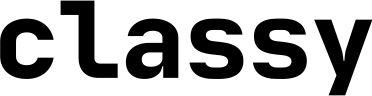
\includegraphics[width=.8\textwidth]{gfx/logo_classy}\\
      \end{column}


    \begin{column}{.7\textwidth}
      \begin{overlayarea}{\textwidth}{\textheight}
        \vspace{1em}

        \begin{itemize}[<.->]
          \item \emph{\bf Spectra are complex data products}
            \begin{itemize}[<.->]
              \item[$\circ$] Wavelength, Reflectance, Irradiance, \dots
              \item[$\circ$] Instrument Metadata
              \item[$\circ$] Sample Metadata
            \end{itemize}
        \vspace{1em}
          \item \emph{\bf Spectra Databases for Ast./Comets/Met.}
            \begin{itemize}[<.->]
              \item[$\circ$] PDS, CDS, RELAB
              \item[$\circ$] SMASS, MITHNEOS
            \end{itemize}
        \vspace{1em}
          \item \emph{\bf Spectra Aggregators for Asteroids and Meteorites}
            \begin{itemize}[<.->]
              \item[$\circ$] SSHADE, M4AST, classy
              \item[$\circ$] Processing required
              \item[$\circ$] Few updates
            \end{itemize}

        \end{itemize}
      \end{overlayarea}
    \end{column}

  \end{columns}

\end{frame}

\begin{frame}[t]{Demo}
  The next slides show an outline of the demoed material.
\end{frame}

\begin{frame}[t]{M4AST}
  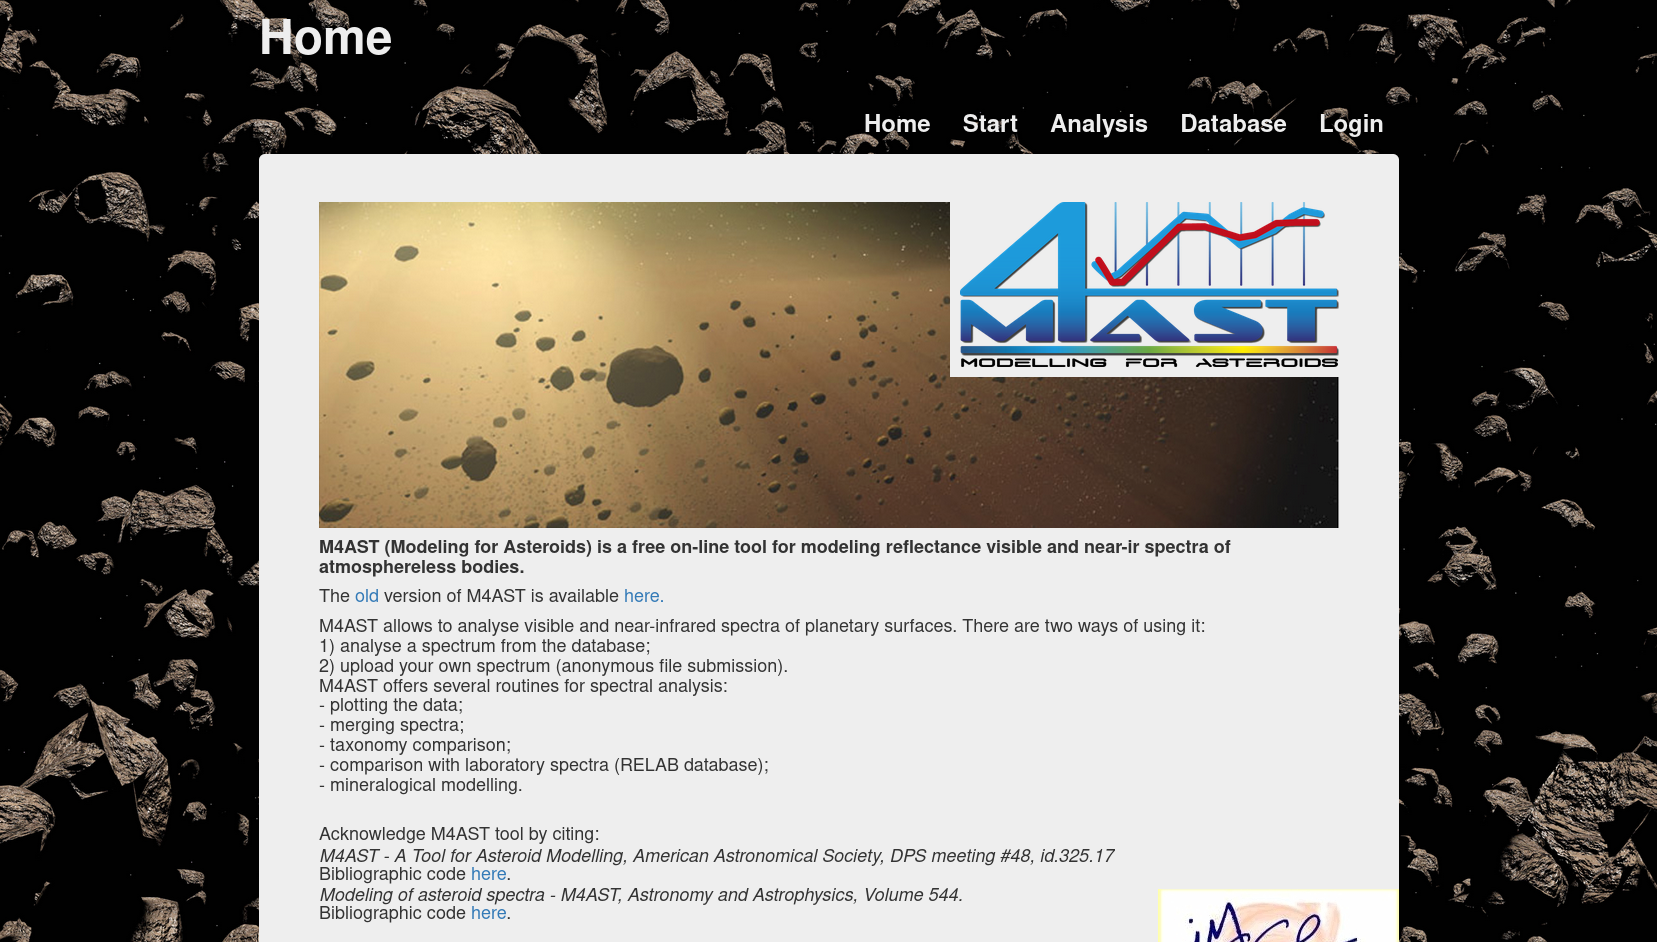
\includegraphics[width=0.8\textwidth]{gfx/demo_m4ast}
  \url{https://spectre.imcce.fr/m4ast/index.php/index/home}
\end{frame}

\begin{frame}[t]{classy}
  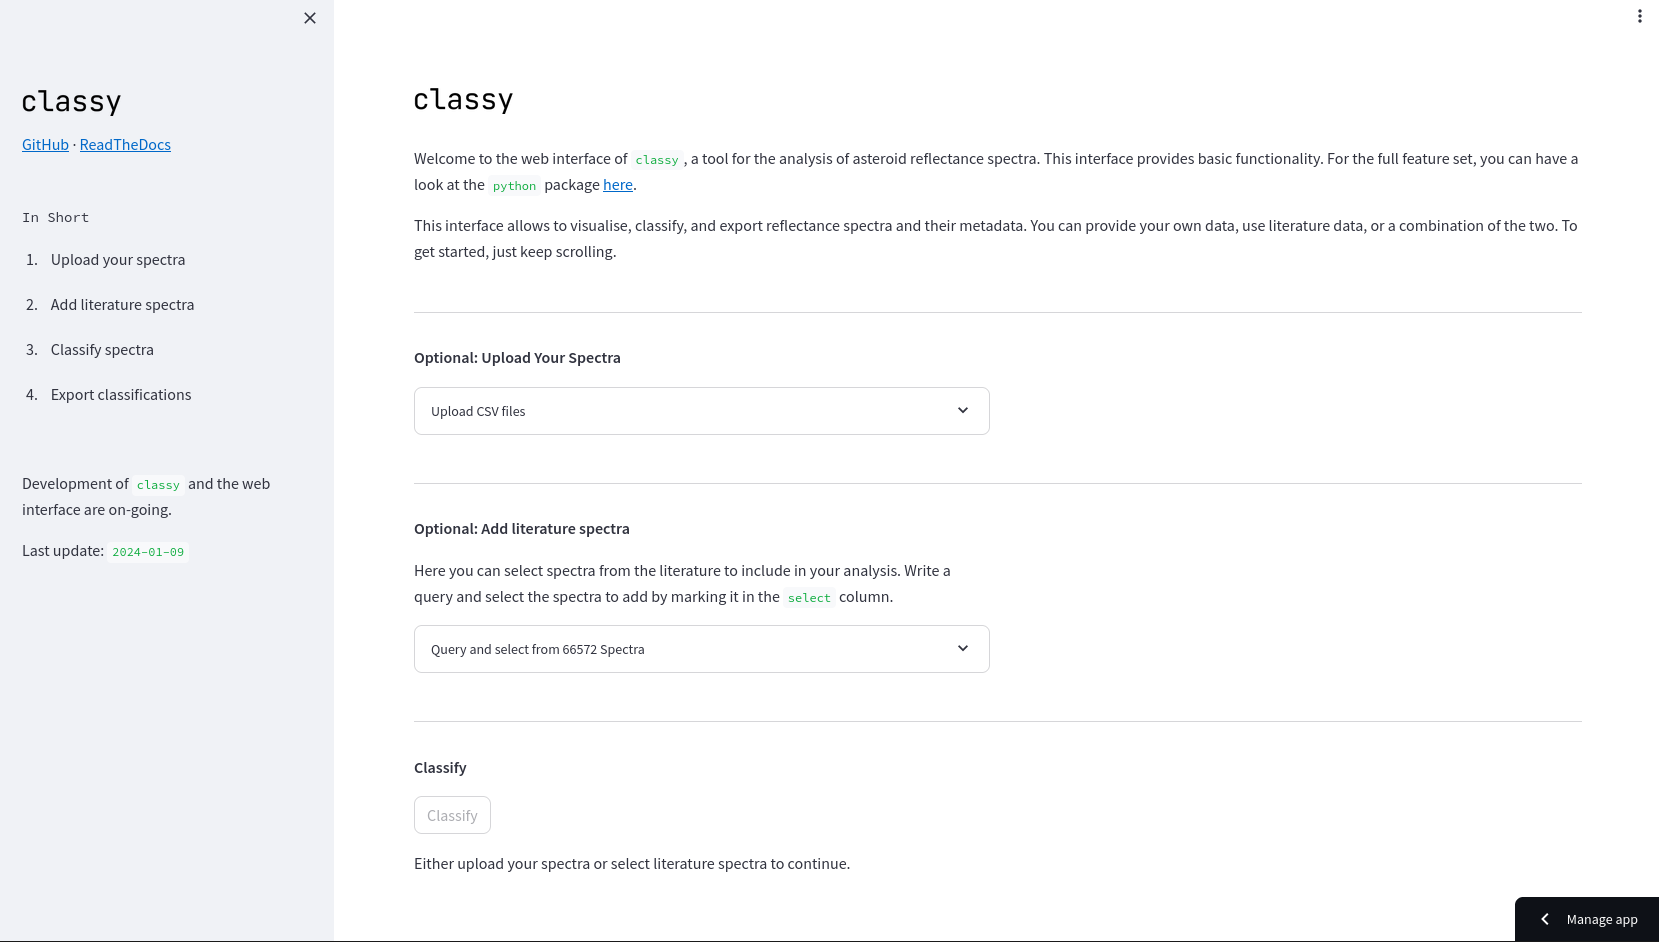
\includegraphics[width=0.8\textwidth]{gfx/demo_classy}
  \url{https://classy.streamlit.app/}
\end{frame}

\begin{frame}[t]{RELAB}
  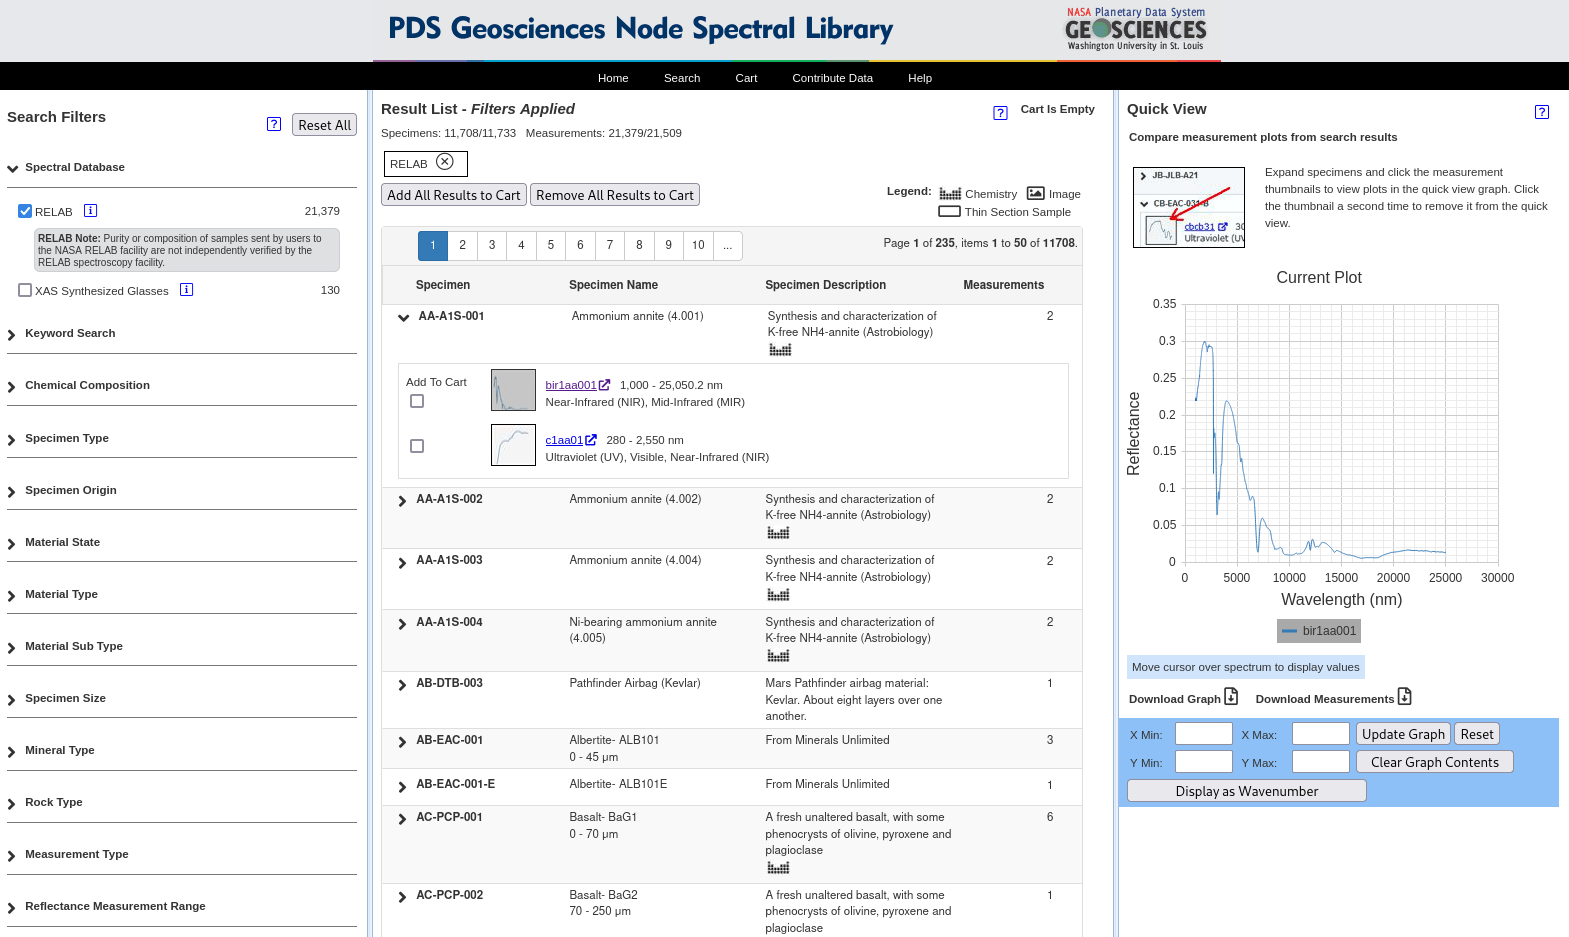
\includegraphics[width=0.8\textwidth]{gfx/demo_relab}
  \url{https://sites.brown.edu/relab/relab-spectral-database/}
\end{frame}

\begin{frame}[t]{SSHADE}
  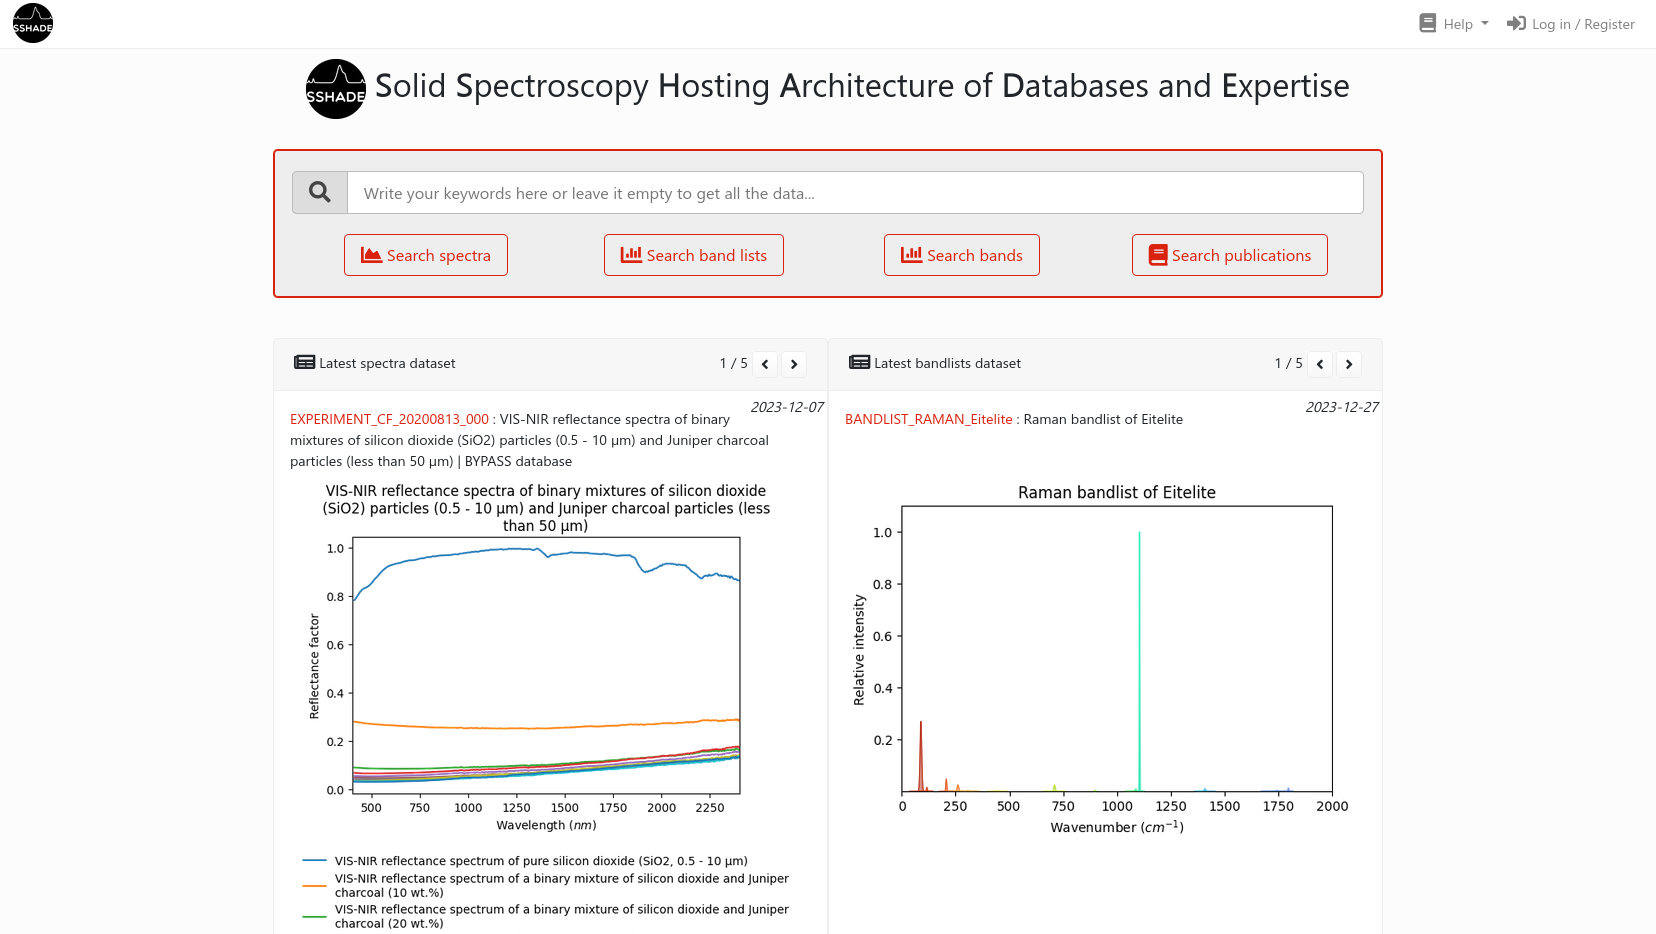
\includegraphics[width=0.8\textwidth]{gfx/demo_sshade}
  \url{https://www.sshade.eu}
\end{frame}

\begin{frame}[t]{SSHADE}
  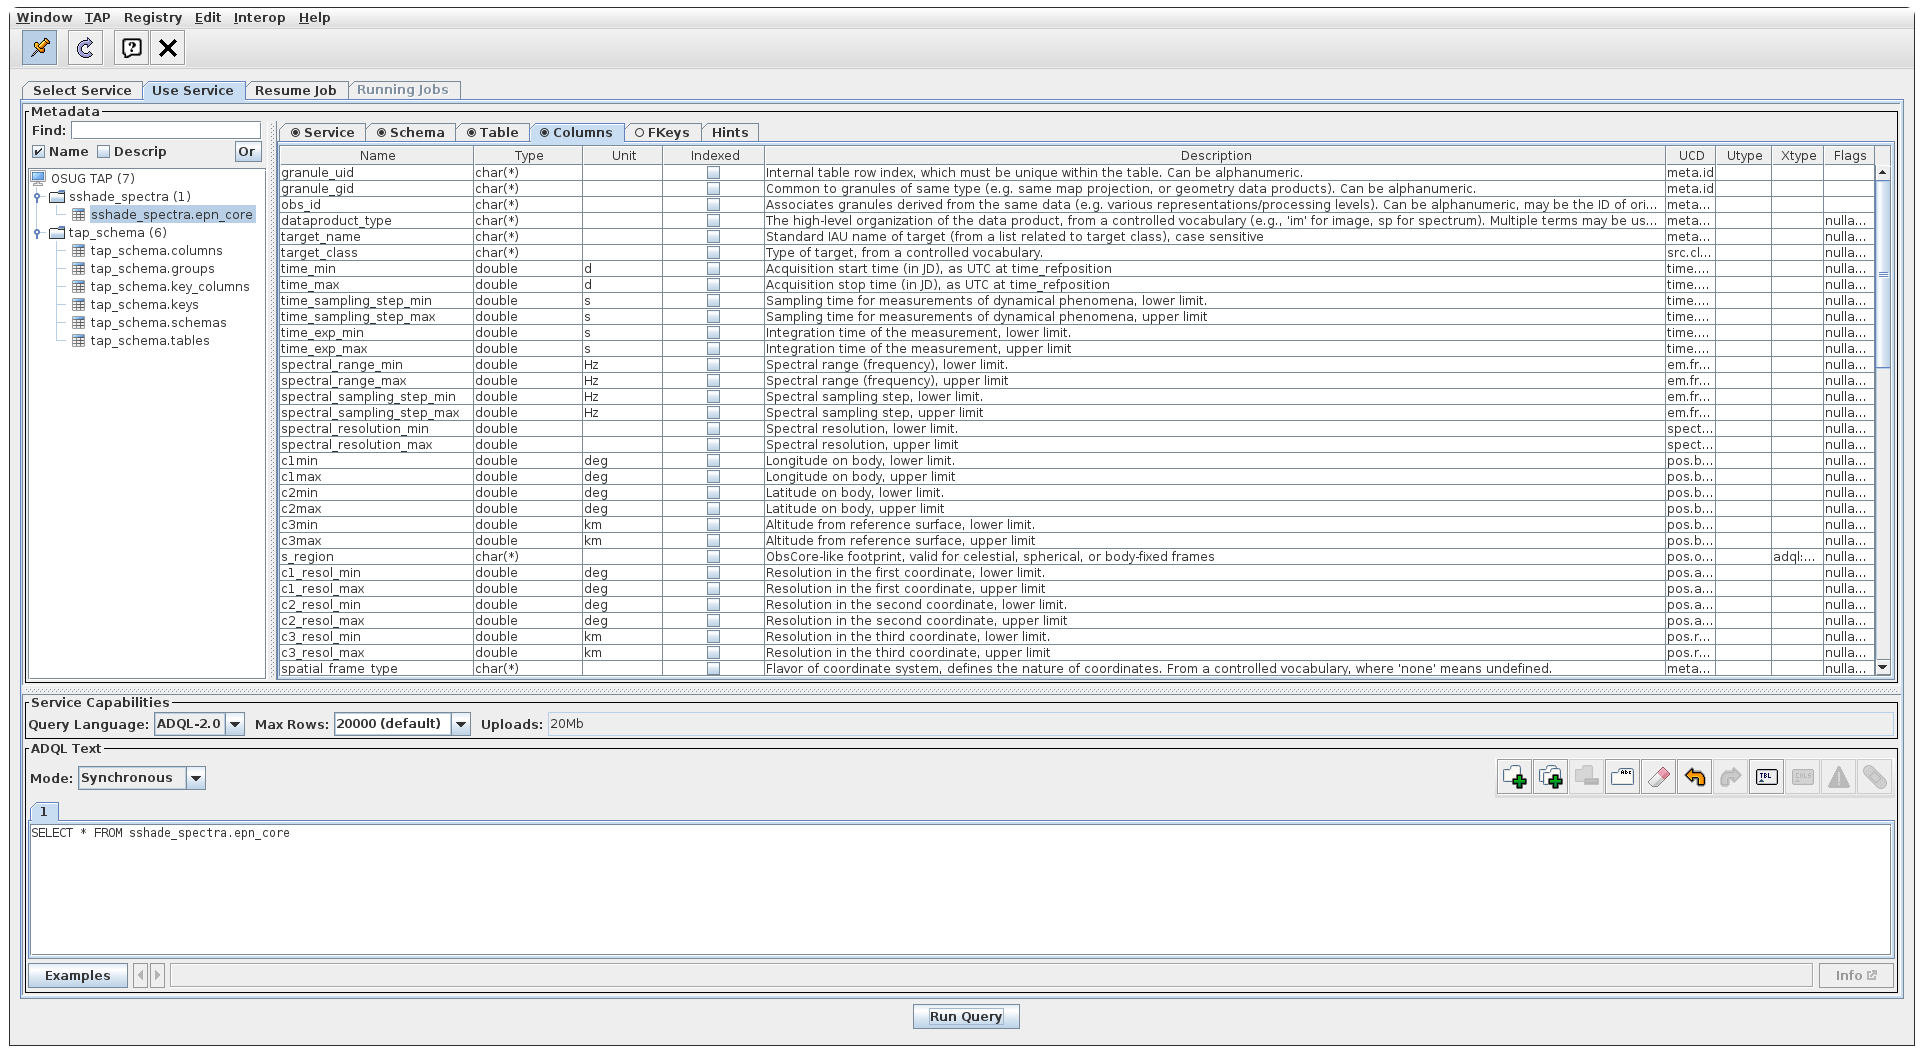
\includegraphics[width=0.8\textwidth]{gfx/demo_tap}\\
  % + missing TAP documentation\\
  % + TAP discovery in TOPCAT
  TOPCAT \textrightarrow~TAP Query \textrightarrow~``SSHADE''
\end{frame}

\begin{frame}[t]{Tutorial}
  [20min] Tutorial notebook on spectra access with SSHADE and TAP
  % Code for classy but without running it [?]
\end{frame}
       % Thursday Part II
  \section{Why shared resources?}


%%%%%%%---- BEGIN ----  ----%%%%%%
\begin{frame}
  \frametitle{A typical research project}

  \begin{columns}[T]

    \begin{column}{.4\textwidth}
      \begin{overlayarea}{\textwidth}{\textheight}
        \only<1>{\hspace{0.05\hsize}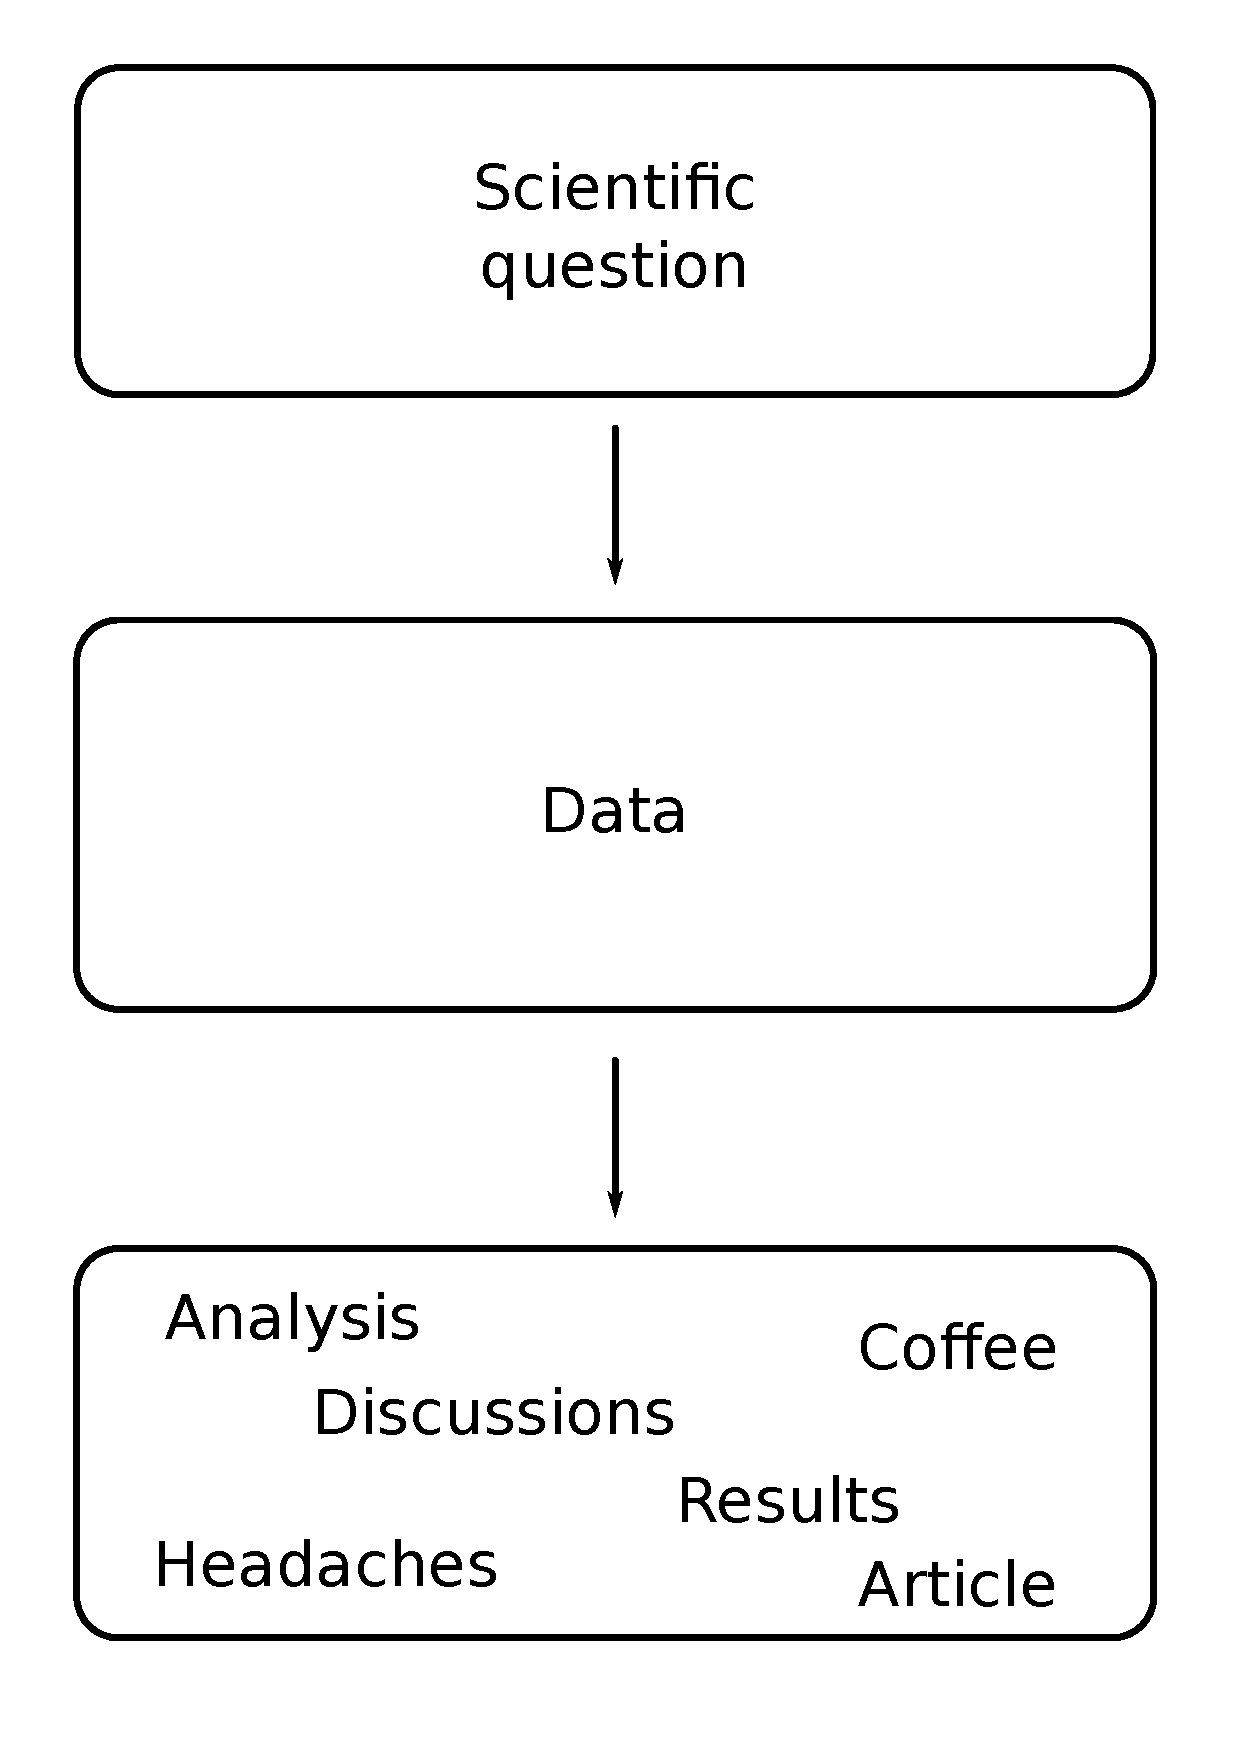
\includegraphics[width=0.9\hsize]{sci_project_1}}
        \only<2>{\hspace{0.05\hsize}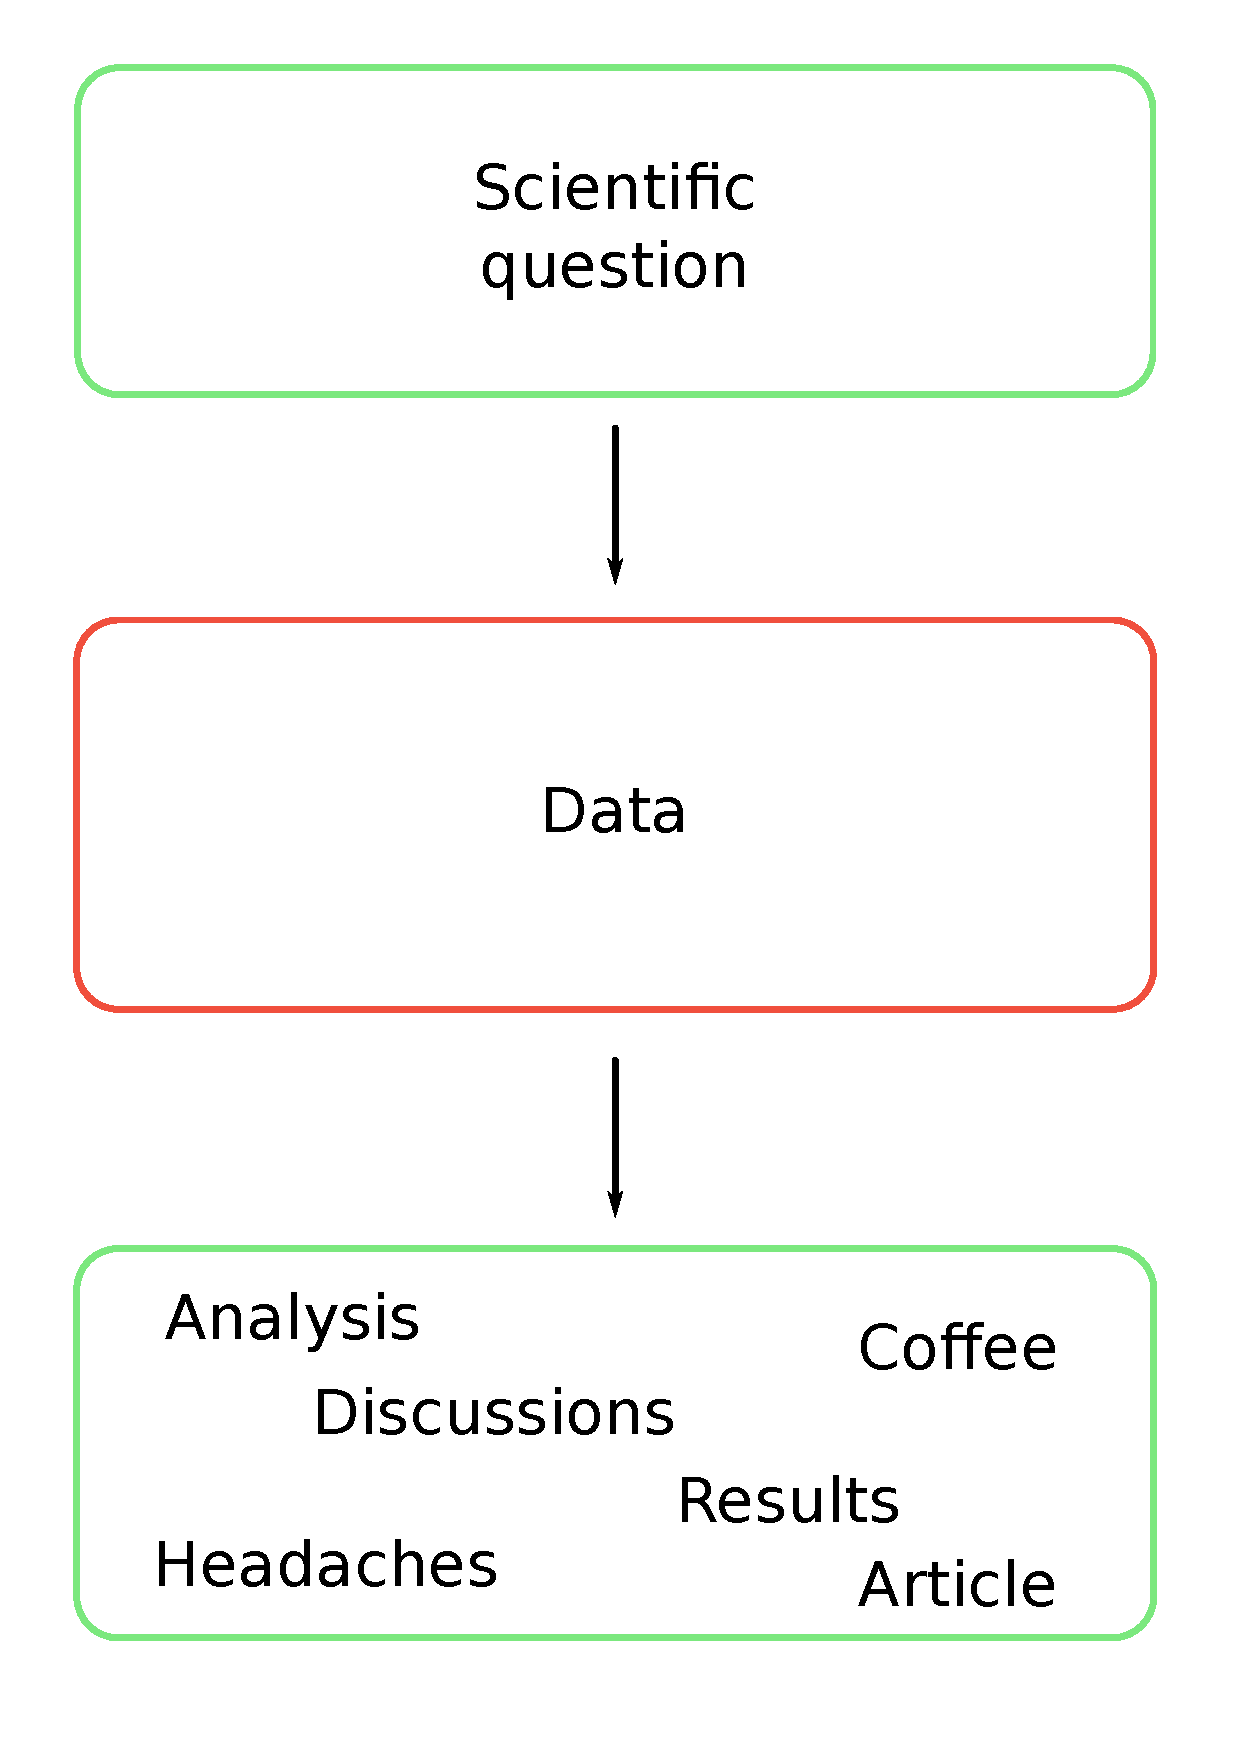
\includegraphics[width=0.9\hsize]{sci_project_2}}
      \end{overlayarea}
    \end{column}


    \begin{column}{.6\textwidth}
      \begin{overlayarea}{\textwidth}{\textheight}
        \begin{onlyenv}<2>

          \vspace{1em}
          \textbf{\bf Repetitive (and tedious) tasks!}\\
          \vspace{1em}
          \begin{itemize}[<.->]
            \item \emph{\bf Planning and conduction of observations}
              \begin{itemize}[<.->]
                \item[$\circ$] Observations already exist?
                \item[$\circ$] Target/sample available? visible?
              \end{itemize}

            \vspace{0.5em}
            \item \emph{\bf Gathering ancillary data for the analysis}
              \begin{itemize}[<.->]
                \item[$\circ$] Complementary information \src{diameter, fall/find, ...}
                \item[$\circ$] Context for research \src{another population}
              \end{itemize}

            \vspace{0.5em}
            \item \emph{\bf Repetitive low-level analysis}
              \begin{itemize}[<.->]
                \item[$\circ$] Spectral classification
                \item[$\circ$] Cross-matches \& merges
              \end{itemize}

          \end{itemize}
        \end{onlyenv}
      \end{overlayarea}
    \end{column}
  
  \end{columns}

\end{frame}
%%%%%%%----  END  ----  ----%%%%%%



%%%%%%%---- BEGIN ----  ----%%%%%%
\begin{frame}
  \frametitle{Shared resources save community time}

  \begin{itemize}[<.->]
    \item \emph{\bf Tedious tasks? Share the load!}
      \begin{itemize}[<.->]
        \item[$\circ$] Many agencies have the mission to support the community
        \item[] \src{ESO/ESA/NASA, JPL/MPC/IMCCE, ...}
        \item[$\circ$] The expertize is in the community $\rightarrow$ individual initiatives
        \item[] \src{SSHADE, Meteoretical Bulletin, SMASS}
        \item[$\blacktriangleright$] More time for your research
      \end{itemize}
  
    \vspace{0.5em}
  \item \emph{\bf Tedious tasks? Automatize them!}
      \begin{itemize}[<.->]
        \item[$\circ$] Click, click, click... copy-paste, click...
        \item[$\circ$] Or code some processes to work for you
        \item[$\blacktriangleright$] Virtual Observatory \& Community librairies
      \end{itemize}
  
    \vspace{0.5em}
    \item \emph{\bf Community services are less prone to errors!}
      \begin{itemize}[<.->]
        \item[$\circ$] One user $\rightarrow$ one $\alpha$-, $\beta$-tester, user...
        \item[$\circ$] Many users $\rightarrow$ bug reports! and community solutions \& patches!
        \item[$\blacktriangleright$] Robustness of analysis $\rightarrow$ results
      \end{itemize}

  \end{itemize}
  
\end{frame}
%%%%%%%----  END  ----  ----%%%%%%




           %-Ok
  \section{Online resources}

%%%%%%%---- BEGIN ----  ----%%%%%%
\begin{frame}
  \frametitle{Online resources in a nutshell}

  \begin{itemize}[<+->]
    \item \emph{A suite of pages, libraries, and services}
      \begin{itemize}[<.->]
        \item[$\circ$] \textbf{Providers:} data archives, catalogs, online codes
        \item[$\circ$] \textbf{Clients:} GUI, CLI, analysis tools
        \item[$\circ$] Check IVOA: \url{http://ivoa.net/astronomers/applications.html}
      \end{itemize}

    \vspace{1em}
    \item \emph{Mostly following a couple of standards}
      \begin{itemize}[<.->]
        \item[$\circ$] Common interface \src{I/O: VOTable, json, Protocols: TAP, cone-search}
        \item[$\circ$] Registries $\rightarrow$ phone book
        \item[$\circ$] Homogeneisation of interface \src{in APIs and in python modules}
      \end{itemize}

    \vspace{1em}
    \item \emph{It is \textbf{not} a master software}

    \vspace{1em}
    \item \emph{Resources are made \textbf{by} us, and \textbf{for} us}
      \begin{itemize}[<.->]
        \item[$\circ$] Powerful libraries and tools
        \item[$\circ$] Good practice to release data/codes \src{Consider CDS at the very least}
        \item[$\circ$] Contribute to open-source projects: \texttt{astroquery}, \texttt{sbpy}, \texttt{rocks}, \dots
      \end{itemize}

  \end{itemize}

\end{frame}
%%%%%%%----  END  ----  ----%%%%%%
        %-

%
\end{document}
